\documentclass[a4paper,11pt]{article}
\usepackage[margin=1.1in]{geometry}
\usepackage[utf8]{inputenc}
\usepackage{graphicx}
\usepackage{booktabs}
\usepackage{minted}
\usepackage[titletoc]{appendix}

%opening
\title{\textbf{Scan chain based test setup for\\ DE0-Nano based systems}}
\author{Advisor : Prof. Madhav P. Desai \\ \\Titto Thomas \\ Wadhwani Electronics Laboratory \\ EE Dept. IIT Bombay}

\begin{document}
\maketitle

%------------------------------------Intro-----------------------------------------------------
\section{Introduction}
Scan chain is a technique used to test the hardware systems. The objective is to make testing easier by providing a simple way to set the inputs and observe the outputs. For simplicity, we can assume them to be a serial in parallel out shift register at the input side and a parallel in serial out shift register at the output side of the Device Under Test (DUT).
\paragraph*{}

Joint Test Action Group (JTAG) is a standard  for testing hardware using scan chains. A simplified version of standard JTAG is proposed here for testing designs on the DE0-Nano board. The system is aimed to test the digital system design, i.e. send input combinations to the hardware and read back their outputs. 


\section{Test Setup}
The complete system has mainly three parts. The first one is a software running on the host PC that gets the command inputs from the user from a text file. Second one is a microcontroller(ATxMega128) that converts the commands (obtained from PC through USB) into a set of signals for the DE0-Nano board. The final one is the DE0-Nano board containing both the DUT and the proposed scan chain.

\begin{figure}[h!]
\centering
% XCircuit output "scan_main.tex" for LaTeX input from scan_main.ps
\def\putbox#1#2#3#4{\makebox[0in][l]{\makebox[#1][l]{}\raisebox{\baselineskip}[0in][0in]{\raisebox{#2}[0in][0in]{\scalebox{#3}{#4}}}}}
\def\rightbox#1{\makebox[0in][r]{#1}}
\def\centbox#1{\makebox[0in]{#1}}
\def\topbox#1{\raisebox{-0.60\baselineskip}[0in][0in]{#1}}
\def\midbox#1{\raisebox{-0.20\baselineskip}[0in][0in]{#1}}
   \scalebox{1}{
   \normalsize
   \parbox{6.75in}{
   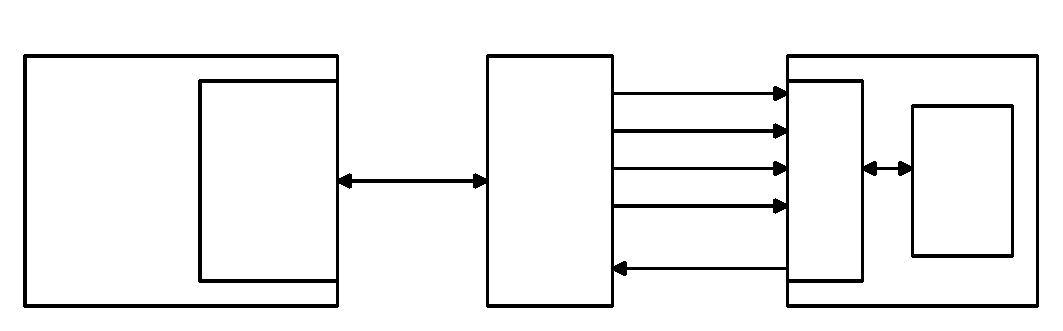
\includegraphics[scale=0.9]{scan_main.eps}\\
   % translate x=1040 y=64 scale 0.38
   \putbox{0.78in}{1.65in}{1.20}{PC}%
   \putbox{2.7in}{1.65in}{1.20}{ATxMega128}%
   \putbox{4.8in}{1.65in}{1.20}{DE0-Nano}%
   \putbox{1.23in}{0.9in}{1.20}{Python}%
   \putbox{1.28in}{0.7in}{1.20}{Script}%
   \putbox{2.02in}{0.6in}{1.20}{USB link}%
   \putbox{3.9in}{1.38in}{1.20}{{\small TDI}}%
   \putbox{3.87in}{1.15in}{1.20}{{\small TCLK}}%
   \putbox{3.9in}{0.92in}{1.20}{{\small TMS}}%
   \putbox{3.87in}{0.68in}{1.20}{{\small TRST}}%
   \putbox{3.9in}{0.11in}{1.20}{{\small TDO}}%
   \putbox{4.8in}{0.35in}{1.20}{\rotatebox{-270}{Scan Chain}}%
   \putbox{5.48in}{0.81in}{1.20}{DUT}%
   } % close 'parbox'
   } % close 'scalebox'
   \vspace{-\baselineskip} % this is not necessary, but looks better
\\
\caption{Block Diagram}
\end{figure}

The user can provide input combinations and their expected outputs in an input text file. The python script will parse the file and extract the commands. The PC communicates to the microcontroller through a USB link , with a predefined standard data transfer scheme. 
\paragraph*{}

The microcontroller will translate the commands, and generate corresponding signals through it's port pins. The hardware description of DUT and the tester hardware are bundled together and implemented on the DE0-Nano board. The tester hardware contains the scan chain and the controller ( TAP controller ) to control it. The interface signals of this top level system would be,

\begin{itemize}
\item \texttt{TDI} : The serial test data input to be loaded in the scan chain.
\item \texttt{TMS} : The commands for the TAP ( Test Access Port ) controller are passed serially through this pin.
\item \texttt{TCLK} : The clock reference forin design for testing all the other communication lines.
\item \texttt{TRST} : Pin to reset the TAP controller at any instant.
\item \texttt{TDO} : The serial data output from the scan chain.
\end{itemize}

%----------------------Adding scan chain to design-----------------------------------------

\section{Adding scan chain to your VHDL design}

The user will have a particular system ( described in VHDL ) that needs to be tested. This DUT should be tested in Gate level simulation and verified to be working, similar to the previous experiments.

Now for testing this DUT, the user have to write a top level entity ( shown as \texttt{mySystem} in fig.2) which uses the DUT as a component. Along with DUT it will also contain \texttt{Scan\_Chain} module as a component, which contains the entire testing hardware. The top level entity will have only these two components communicating with each other.
\texttt{mySystem} should have 5 interface signals (1 bit each) \texttt{TDI}, \texttt{TMS}, \texttt{TCLK}, \texttt{TRST} and \texttt{TDO}.
\begin{figure}[h!]
\centering
% XCircuit output "DUT.tex" for LaTeX input from DUT.ps
\def\putbox#1#2#3#4{\makebox[0in][l]{\makebox[#1][l]{}\raisebox{\baselineskip}[0in][0in]{\raisebox{#2}[0in][0in]{\scalebox{#3}{#4}}}}}
\def\rightbox#1{\makebox[0in][r]{#1}}
\def\centbox#1{\makebox[0in]{#1}}
\def\topbox#1{\raisebox{-0.60\baselineskip}[0in][0in]{#1}}
\def\midbox#1{\raisebox{-0.20\baselineskip}[0in][0in]{#1}}
   \scalebox{1}{
   \normalsize
   \parbox{6.66667in}{
   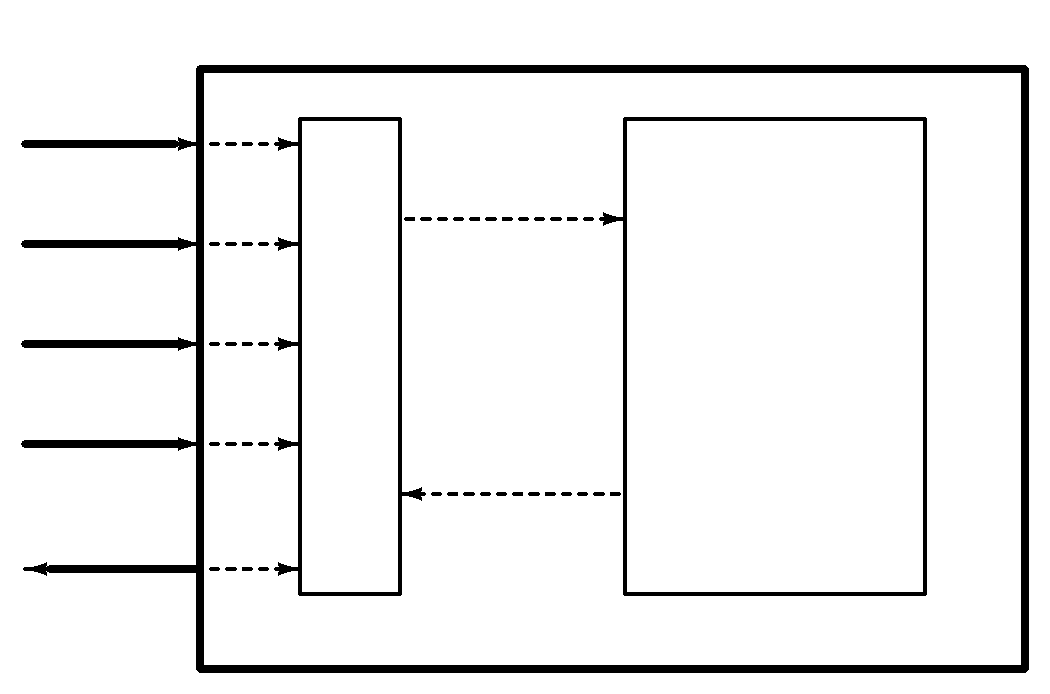
\includegraphics[scale=0.75]{DUT.eps}\\
   % translate x=1024 y=352 scale 0.38
   \putbox{3.59in}{1.56in}{1.20}{DUT}%
   \putbox{2.19in}{2.46in}{1.20}{dut\_in}%
   \putbox{2.19in}{0.66in}{1.20}{dut\_out}%
   \putbox{0.35in}{2.72in}{1.20}{TDI}%
   \putbox{0.27in}{2.22in}{1.20}{TCLK}%
   \putbox{0.31in}{1.73in}{1.20}{TMS}%
   \putbox{0.22in}{1.22in}{1.20}{TRST}%
   \putbox{0.31in}{0.6in}{1.20}{TDO}%
   \putbox{1.58in}{1.16in}{1.20}{\rotatebox{-270}{Scan Chain}}%
   \putbox{3.94in}{3.12in}{1.20}{mySystem}%
   } % close 'parbox'
   } % close 'scalebox'
   \vspace{-\baselineskip} % this is not necessary, but looks better
\\
\caption{Scan chain added with DUT}
\end{figure}

All the interface signals of \texttt{mySystem} should be directly connected to the scan chain module as shown in fig.2. 
\paragraph*{}

The scan chain module has two configurable parameters ( \texttt{in\_pins} and \texttt{out\_pins} ) indicating the number of input and output bits to the DUT, which can be generic mapped. It also has one output (\texttt{dut\_in}) and one input (\texttt{dut\_out}) that should be connected to the DUT. Internally it contains an FSM ( \textit{TAP Controller} ), one input scan register ( \textit{In Register} ) and one output scan register ( \textit{Out Register} ). The diagram showing the details of scan chain module is given in fig.3 and the entity of the scan chain module is given below.

\begin{minted}{vhdl}
entity Scan_Chain is
  generic (
    in_pins : integer; -- Number of input pins
    out_pins : integer -- Number of output pins
  );
  port (
    TDI : in std_logic;  -- Test Data In
    TDO : out std_logic;  -- Test Data Out
    TMS : in std_logic;  -- TAP controller signal
    TCLK : in std_logic;  -- Test clock
    TRST : in std_logic;  -- Test reset
    dut_in : out std_logic_vector(in_pins-1 downto 0);  -- Input for the DUT
    dut_out : in std_logic_vector(out_pins-1 downto 0);  -- Output from the DUT
  );
end Scan_Chain;
\end{minted}

%----------------------Reference Implementation-----------------------------------------
\section{Reference Implementation}

\begin{figure}[h!]
\centering
% XCircuit output "Counter.tex" for LaTeX input from Counter.ps
\def\putbox#1#2#3#4{\makebox[0in][l]{\makebox[#1][l]{}\raisebox{\baselineskip}[0in][0in]{\raisebox{#2}[0in][0in]{\scalebox{#3}{#4}}}}}
\def\rightbox#1{\makebox[0in][r]{#1}}
\def\centbox#1{\makebox[0in]{#1}}
\def\topbox#1{\raisebox{-0.60\baselineskip}[0in][0in]{#1}}
\def\midbox#1{\raisebox{-0.20\baselineskip}[0in][0in]{#1}}
   \scalebox{1}{
   \normalsize
   \parbox{5.16667in}{
   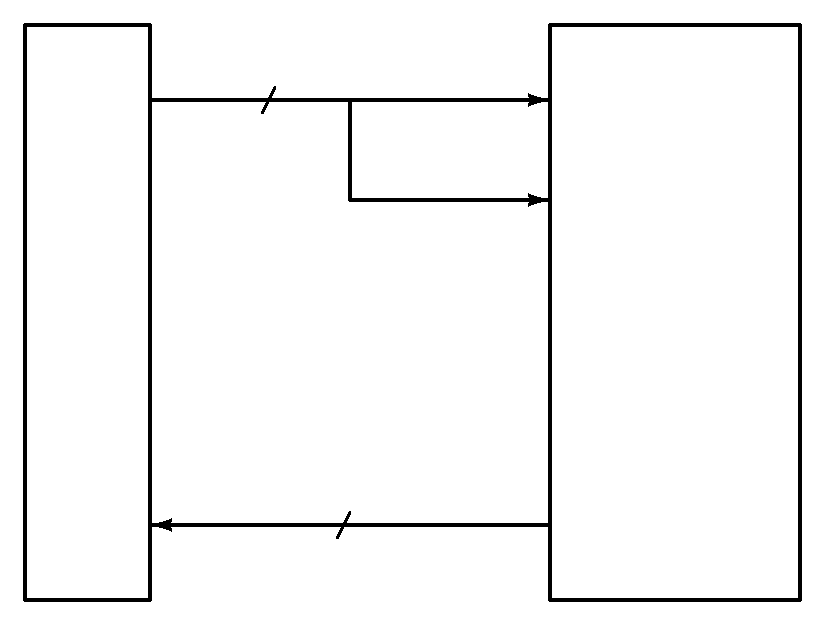
\includegraphics[scale=0.8]{Counter.eps}\\
   % translate x=672 y=512 scale 0.38
   \putbox{0.78in}{2.86in}{1.20}{\texttt{dut\_in[1:0]}}%
   \putbox{1.97in}{2.86in}{1.20}{\texttt{dut\_in[1]}}%
   \putbox{1.97in}{2.32in}{1.20}{\texttt{dut\_in[0]}}%
   \putbox{1.36in}{0.62in}{1.20}{\texttt{dut\_out[7:0]}}%
   \putbox{2.94in}{0.4in}{1.20}{\texttt{count}}%
   \putbox{2.94in}{2.65in}{1.20}{\texttt{reset}}%
   \putbox{2.94in}{2.1in}{1.20}{\texttt{clock}}%
   \putbox{0.35in}{1.16in}{1.20}{\rotatebox{-270}{Scan Chain}}%
   \putbox{3.2in}{1.4in}{1.20}{Counter}%
   } % close 'parbox'
   } % close 'scalebox'
   \vspace{-\baselineskip} % this is not necessary, but looks better
\\
\caption{Connecting Counter to the scan chain}
\end{figure}

The reference implementation given here is that of a counter. The counter has two single bit inputs ( \texttt{clock} and \texttt{reset} ) and an 8 bit single output ( \texttt{count}). Here, the \texttt{dut\_in} will be 2 bits ( one for each of the inputs ) and \texttt{dut\_in} will be same as \texttt{count}. The connections are clearly shown in fig. 3.
\paragraph*{}
The top level VHDL description of this system is given in Appendix I.



%---------------------- Hardware Connections -----------------------------------------

\section{Hardware connections}
Next step is to make physical connections between the host PC, microcontroller board and the user module( on DE0-Nano). The microcontroller board is PtX-128 ( ATxMega128 based ) developed in WEL lab, IITB. The following connections between the microcontroller board and the DE0-Nano need to be made.

\begin{itemize}
\item Connect \texttt{TRST} (DE0-Nano) to PD4 (PORTD.4)
\item Connect \texttt{TDI} (DE0-Nano) to PD0 (PORTD.0)
\item Connect \texttt{TMS} (DE0-Nano) to PD1 (PORTD.1)
\item Connect \texttt{TCLK} (DE0-Nano) to PD5 (PORTD.5)
\item Connect \texttt{TDO} (DE0-Nano) to PC0 (PORTC.0)
\end{itemize}

Also connect the PtX-128 board to the host machine using the USB cable provided.

%---------------------- Input file format -----------------------------------------
\section{Test vector file format}
For testing the hardware, the user has to provide input combinations, their expected results and the time duration of execution. They should be written as commands in a text file and passed to the python script for test execution. These commands are derived from the SVF format, usually used in JTAG boundary scan. The inputs commands ( a subset of standard SVF commands ) are given below. Only two commands are required for the current implementation.

\begin{itemize}
 \item \texttt{SDR $<in\:pins>$ TDI($<input>$) $<out\:pins>$ TDO($<output>$) MASK($<mask\:bits>$)}
	\vspace*{0.3cm}
	\newline This Serial Data Register instruction is for carrying out a data scan in process. $in\:pins$ \& $out\:pins$ contains the number of input and output bits respectively. Similarly, $input$ \& $output$ contains the input combination to be applied and it's expected output combination respectively. $mask\:bits$ are used to specify if any of the output bits are not important and could be taken as don't care ( if one bit is 0 then the corresponding output bit is taken as don't care ).\\\\
Example : \texttt{SDR 2 TDI(0) 8 TDO(00) MASK(FF)}
\\\\
\textit{Note} : If the scanned output should not be compared, then all the $mask\:bits$ should be kept as 0.
 \item \texttt{RUNTEST $<delay>$ SEC} :
	\vspace*{0.3cm}
	\newline As the previous instruction loads the input and samples the output, this instruction is used to apply the input combination to the DUT and wait for $delay$ seconds.\\\\
Example : \texttt{RUNTEST 60 SEC}
\end{itemize}

The $input$, $output$ and $mask\:bits$ are to be written as hexadecimel numbers ( uppercase for alphabets ). An example input file is given in the Appendix II.

%---------------------- Running python script -----------------------------------------
\section{Running the Python script}
Before running the python script, pyUSB library needs to be installed on the PC by the following steps.

\begin{itemize}
\item Download pyUSB v1.0 from the site ``\textit{http://sourceforge.net/projects/pyusb/}"
\item Follow the steps in the README document to install libusb and pyusb v1.0 on linux machine.
\end{itemize}

After the installation run the \texttt{scan.py} script with the following command.
\begin{center}
\texttt{\$ sudo scan.py \textit{<input file>} \textit{<output file>}} 
\end{center}

Where the \textit{input file} should contain all the commands to be executed, and \textit{output file} should be an empty file ( already created by the user ) for storing the results back.


%---------------------- Appendix -----------------------------------------

\newpage
\section*{Appendix I}
\begin{minted}{vhdl}
library ieee;
use ieee.std_logic_1164.all;
use ieee.std_logic_unsigned.all;

entity mySystem is
  port (
    clock_50 : in std_logic;
    TDI : in std_logic;  -- Test Data In
    TDO : out std_logic;  -- Test Data Out
    TMS : in std_logic;  -- TAP controller signal
    TCLK : in std_logic;  -- Test clock
    TRST : in std_logic;  -- Test reset
    LED : out std_logic_vector(7 downto 0)  -- LED outputs for checking
  );
end mySystem;

architecture behave of mySystem is

component Scan_Chain is	-- Scan Chain as a component
  generic (
    in_pins : integer; -- Number of input pins
    out_pins : integer -- Number of output pins
  );
  port (
    TDI : in std_logic;  -- Test Data In
    TDO : out std_logic;  -- Test Data Out
    TMS : in std_logic;  -- TAP controller signal
    TCLK : in std_logic;  -- Test clock
    TRST : in std_logic;  -- Test reset
    dut_in : out std_logic_vector(in_pins-1 downto 0);  -- Input for the DUT
    dut_out : in std_logic_vector(out_pins-1 downto 0);  -- Output from the DUT
  );
end component;

component Counter is
  port (
    clock : in std_logic;  -- Clock signal
    reset : in std_logic;  -- Reset signal
    count : out std_logic_vector(7 downto 0)  -- Counter output
    );
end component;

signal dut_in : std_logic_vector(1 downto 0);
signal dut_out : std_logic_vector(7 downto 0);
signal reset, clock : std_logic;

begin  -- behave

 reset <= dut_in(1);  -- seperating the DUT input signals
 clock <= dut_in(0);

-- Connect the scan chain for testing 
 SC : Scan_Chain generic map (2,8) port map ( TDI,TDO,TMS,TCLK,TRST,dut_in,dut_out );

 DUT: Counter port map (clock, reset, dut_out); -- Connect DUT
  
end behave;
\end{minted}

\section*{Appendix II}
SDR 2 TDI(2) 8 TDO(00) MASK(00)\\
RUNTEST 60 SEC\\
SDR 2 TDI(0) 8 TDO(00) MASK(00)\\
RUNTEST 60 SEC\\
SDR 2 TDI(1) 8 TDO(00) MASK(00)\\
RUNTEST 60 SEC\\
SDR 2 TDI(0) 8 TDO(00) MASK(00)\\
RUNTEST 60 SEC\\
SDR 2 TDI(1) 8 TDO(00) MASK(00)\\
RUNTEST 60 SEC\\
SDR 2 TDI(0) 8 TDO(00) MASK(00)\\
RUNTEST 60 SEC\\
SDR 2 TDI(1) 8 TDO(00) MASK(00)\\
RUNTEST 60 SEC\\
SDR 2 TDI(0) 8 TDO(00) MASK(00)\\
RUNTEST 60 SEC\\
SDR 2 TDI(1) 8 TDO(00) MASK(00)\\
RUNTEST 60 SEC\\
SDR 2 TDI(0) 8 TDO(00) MASK(FF)\\
RUNTEST 60 SEC\\
\end{document}